\chapter{Stand van zaken}
\label{ch:stand-van-zaken}

% Tip: Begin elk hoofdstuk met een paragraaf inleiding die beschrijft hoe
% dit hoofdstuk past binnen het geheel van de bachelorproef. Geef in het
% bijzonder aan wat de link is met het vorige en volgende hoofdstuk.

% Pas na deze inleidende paragraaf komt de eerste sectiehoofding.

% Dit hoofdstuk bevat je literatuurstudie. De inhoud gaat verder op de inleiding, maar zal het onderwerp van de bachelorproef *diepgaand* uitspitten. De bedoeling is dat de lezer na lezing van dit hoofdstuk helemaal op de hoogte is van de huidige stand van zaken (state-of-the-art) in het onderzoeksdomein. Iemand die niet vertrouwd is met het onderwerp, weet er nu voldoende om de rest van het verhaal te kunnen volgen, zonder dat die er nog andere informatie moet over opzoeken \autocite{Pollefliet2011}.

% Je verwijst bij elke bewering die je doet, vakterm die je introduceert, enz. naar je bronnen. In \LaTeX{} kan dat met het commando \texttt{$\backslash${textcite\{\}}} of \texttt{$\backslash${autocite\{\}}}. Als argument van het commando geef je de ``sleutel'' van een ``record'' in een bibliografische databank in het Bib\TeX{}-formaat (een tekstbestand). Als je expliciet naar de auteur verwijst in de zin, gebruik je \texttt{$\backslash${}textcite\{\}}.
% Soms wil je de auteur niet expliciet vernoemen, dan gebruik je \texttt{$\backslash${}autocite\{\}}. In de volgende paragraaf een voorbeeld van elk.

% \textcite{Knuth1998} schreef een van de standaardwerken over sorteer- en zoekalgoritmen. Experten zijn het erover eens dat cloud computing een interessante opportuniteit vormen, zowel voor gebruikers als voor dienstverleners op vlak van informatietechnologie~\autocite{Creeger2009}.

% \lipsum[7-20]



Redhat rapporteert dat Meltdown en Spectre tezamen een impact van 0 tot 19 procent heeft.
Applicaties die vaak systeemoproepen doen zullen meer prestatieverlies hebben. 
De grootste verliezers zijn database workloads die veel gebruik maken van willekeurige data in de cache zoals sysbench, pgbench (voorheen 8 tot 19 procent, nu bijgewerkt met retpoline naar 4 tot 8 procent).
Applicaties die weinig nood hebben aan kernelgeheugen zoals HPC (High Performance Computing) met OpenMP hebben weinig last van Spectre en Meltdown. Het verschil was eerst 2 tot 5 procent maar met betere updates is het gedaald naar 1 tot 2 procent.



\autocite{Redhat2018}






%\chapter{}
%\section{ }

\chapter{Achtergrond}



\section{Spectre}

\subsection{Spectre aanval}
Spectre is geclassificeerd als een 'side channel aanval'.
Een side channel aanval is een verzameling van aanvallen op een cryptografie apparaat met als doel de geheime sleutel ervan te onthullen.

De aanvaller probeert bepaalde patronen in het systeem te ontdekken door analyse van informatie die is verkregen uit de fysieke implementatie van het systeem. Deze informatie kan bijvoorbeeld timingsanalyse, stroomverbruik, elektromagnetische lekken of zelfs geluid zijn. \parencite{Touhafi2011}
Computers zijn niet alleen vatbaar voor fysieke side channel aanvallen.

Microprocessors met kwetsbare speculatieve executie mogelijkheden zijn gevonden in miljarden toestellen van Intel, AMD en ARM.

Ook Intel SGX (Sofware Guard eXtensions) is vatbaar voor Spectre. 
Het doel van Intel SGX is om het vertrouwensvereiste tussen gebruiker en een clouddienst zoals Amazon te verminderen.

Het biedt een praktische platformabstractie aan om de programmeur te helpen. 
Het is een soort van beveiligde DRM (Digital Rights Management).
Intel SGX maakt een container aan die software isoleert van andere software.
Dit betekent niet dat men Amazon of Intel 100 procent kan vertrouwen (ze kunnen extreem moeilijk garanderen dat ze geen backdoor voor het debuggen van SGX geïnstalleerd hebben).
Een aantal onderzoekers hebben nu met een Spectre aanval data in de Intel SGX kunnen lezen.
Ze hebben 'SGXPECTRE'  losgelaten op de SGX 'enclave' (enclaves zijn privéregio's van geheugen) om de geheimen er uit te halen.

Om de werking in praktijk te tonen, hebben ze systematisch de mogelijke vectoren van 'branch target injection' onderzocht om de raceconditie te winnen tijdens de speculatieve uitvoering van de enclave. Verder is er onderzocht naar technieken om automatisch codepatronen te vinden nodig voor een aanval te lanceren. Praktische aanvallen zijn mogelijk tegen een willekeurig  enclaveprogramma geschreven met Intel's SGX SDK. Niet alleen kunnen geheimen gelezen worden in het enclave-geheugen, maar ook de registers die in enclave-modus in gebruik zijn \parencite{Chen2018}.

Er wordt wel benadrukt dat er fysieke toegang nodig is tot het systeem. Met fysieke toegang zou Indirect Branch Restricted Speculation (IBRS) uitgeschakeld kunnen worden die geïnstalleerd is met een patch.
De enclave controleert nog niet of IBRS is ingeschakeld.

De aanval is ongeveer gelijk met de branch misprediction Spectre aanval van Kocher et al. \parencite{Kocher2018}. Het enige verschil is dat de geheime gegevens, de slachtofferfunctie (victim\_function) en de overflowarray in de enclave verplaatst worden.
Een array overflow gebeurt wanneer er geprobeerd wordt gegevens in een array te schrijven en de gegevens de grootte van de array overschrijdt.
De aanvaller roept 'victim\_function' aan via een 'ecall' om de array te indexeren. \parencite{Tian2018}

\subsection{Spectre Next Generation}
Begin mei 2018 zijn acht nieuwe kwetsbaarheden gevonden die 'Spectre Next Generation' genoemd worden door c't \parencite{Schmidt2018}. Intel is er al een tijdje van op de hoogte.
Vier ervan worden beschouwd als 'kritiek' en de indentificatienummers zijn al toegewezen in de CVE (Common Vulnerabilities and Exposures) database.

De andere vier worden als medium-risk gecategoriseerd.
Eén van de lekken is zeer kritiek omdat het hostsysteem aangevallen kan worden vanuit een virtuele machine. Dit is een probleem voor cloud-providers zoals Amazon AWS (Amazon Web Services).
De nieuwe kwetsbaarheden hebben zeker ook invloed op AMD-processors.
Intel beweert dat Spectre NG al wordt ondersteund door de bestaande patch maar Microsoft gaat een cumulatieve update uitbrengen.

De aanvallen richten zich op SMM (System Management Mode) in de SMRAM.
SMM is een speciale x86 processor modus dat kernels of hypervisors niet kunnen lezen of wijzigen \parencite{Delgado2013}.
Spectre en Meltdown hebben invloed op software, kernels, hypervisors en zelfs Intel SGX enclaves, maar niet op firmware zoals BIOS of UEFI.


\subsection{Patch}
Spectre is meer ingrijpend als Meltdown.
Intel heeft Skylake (6000-series) definitief gepatched.
Intel had al een bèta-patch maar die veroorzaakte spontane reboots en de distributie is ervan stopgezet.

Kaby Lake (7000-series) en Coffee Lake (8000-series) hebben definitieve microcode patches gekregen. De vorige bèta patches hadden ook veel bugs.

De moederbordfabrikanten moeten die nu in hun bios implementeren.

Voor de volledige roadmap heeft Intel de 'Microcode Revisions Guidance' online gezet.

Volgens die roadmap gaat Intel door tot Core 2 Duo/Quad uit 2008.
Ondertussen heeft Intel het werk aan de patches voor oudere processorseries stopgezet.
Het gaat over de eerste generatie Core i7/i5 processors (de Bloomfield-generatie) en sommige chips van de Core 2 Duo en Core 2 Quad generatie.


Als verklaring geeft Intel: ``Na een uitgebreid onderzoek naar de microarchitectuur en microcodemogelijkheden voor deze producten, heeft Intel besloten geen microcode-updates voor deze producten vrij te geven voor één of meer redenen, waaronder, maar niet beperkt tot het volgende:

a) Micro - architecturale kenmerken die een praktische implementatie van Variant 2 (CVE - 2017 - 5715) uitsluiten;

b) Beperkte ondersteuning van systeemsoftware;

c) Op basis van feedback worden de meeste van deze producten geïmplementeerd als 'gesloten systemen' en daarom wordt verwacht dat ze een lagere kans hebben om te worden blootgesteld aan deze kwetsbaarheden''  \parencite{Intel2018a}.


Maar het valt nog te zien of moederbordfabrikanten een nieuwe BIOS voorzien met de gepatchte microcode.

Volgens Intel CEO Brian Krzanich zullen de volgende generatie Intel CPU's een hardwarematige fix hebben. De bron van Spectre (branch prediction en speculative execution) zal nog steeds werken en snelheidswinst geven, maar de processorarchitectuur zal moeten aangepast worden.

De microcode in een patch wordt niet direct weggeschreven naar de processor maar wordt gewoon bij elke boot opnieuw ingeladen.

Goede oplossingen vereisen veranderingen in processor ontwerpen en architectuur (Instruction Set Architectures).

Bestuursvoorzitter van AMD 'Lisa Su' heeft aangekondigd dat de Zen 2-processors (Ryzen 3000-serie), die vermoedelijk in Q1 van 2019 uitkomen op hardwarelevel tegen Spectre zullen beveiligd zijn. Ryzen 2, die in april 2018 uitgekomen zijn, zijn niet uitgerust met zo een update. Microcode-updates voor al de processors in de serie zijn natuurlijk wel beschikbaar.

De processors van Intel krijgen vanaf eind 2018 al hardwarematige oplossingen voor Meltdown en Spectre.
Dit heeft Brian Krzanich (CEO van Intel) aan zijn investeerders laten weten tijdens de publicatie van de financiën van Intel. Krzanich belooft dat de nieuwe chips (die vermoedelijk op het 10 nm-procedé werken) bestendig zullen zijn tegen Meltdown/Spectre.

Patches voor Page Table Isolation (PTI) tegen Meltdown zijn er al sinds het begin van dit jaar. De patches zijn nu verfijnd en zelfs de 32-bits versie is geïmplementeerd voor x86-systemen.
Patches voor Windows waren niet zonder problemen: een bug in de Meltdown patch zorgde voor een kernelgeheugenlek zonder enige exploitatie en kon door één ieder gelezen worden.

Ook voor System Z van IBM zijn er patches voor beide Spectre versies.
In plaats van Retpoline noemt de patch 'Expoline'.
Retpoline is niet mogelijk omdat op System Z systemen er geen 'return' instructies zijn maar indirecte branches voor de return functies. Expoline code roept nu indirecte branch instructies aan via EX en EXRL instructies.

ARM 64-bit systemen in smartphones zijn beschermd voor Spectre v1, v2 en Meltdown.

Spectre variant 1 heeft alleen invloed op het lokaal proces.
De patch voor variant 1 is een risicobeperkende maatregel voor de output van compilers aan te passen.

Sinds Spectre gebruik kan maken van Javascript hebben alle grote browsers een update gekregen.
Google gebruikt met Chrome 'Site isolation'. Site isolation zorgt ervoor dat elke site een verschillend proces krijgt toegewezen. Zo hebben ze alleen maar toegang tot hun eigen data.

\subsection{Branch Prediction Units}
Branch Prediction Units (BPU) zorgen ervoor dat de microprocessor ononderbroken instructieopdrachten krijgt.
Ze sturen die opdrachten door de executiepijplijn met meerdere voorwaardelijke branches.
Voor elke fysieke kern is er één BPU.
Dit wil zeggen dat meerdere processen worden uitgevoerd op dezelfde BPU.
Hoewel dit interessant is voor complexiteit kan het gemakkelijk gemanipuleerd worden.
Het delen maakt een side channel aanval mogelijk.

Op de meeste chips is de BPU samengesteld uit de branch target buffer (BTB) en de directionele predictor.
Een typische predictor is een simpele enkelvoudige bimodale predictor.
Een enkelvoudige predictor maakt gebruik van directe mapping en alleen het branch adres als bron.
Het neemt de \emph{n}-laatste bits van een branch instructie adres en mapt het in een tabel met een enkele kolom. In de tabel passen 2\textsuperscript{n} rijen.
Op de Haswell gebaseerde Surface Pro 3 worden de laatste bits van het virtuele adres
verder gereduceerd door een eenvoudige hash
functie.

Elke rij bestaat in het algemeen uit een bit-teller (n-bit counter).
De teller is in de meeste gevallen ontworpen als een verzadigde teller (saturated counter).
Er zijn 1-bit en 2-bit verzadigde tellers.
Een 1-bit verzadigde teller registreert de laatste uitkomst van de branch.
Een simpelere teller dan deze is er niet en het is ook niet effectief of efficiënt.


\begin{figure}
	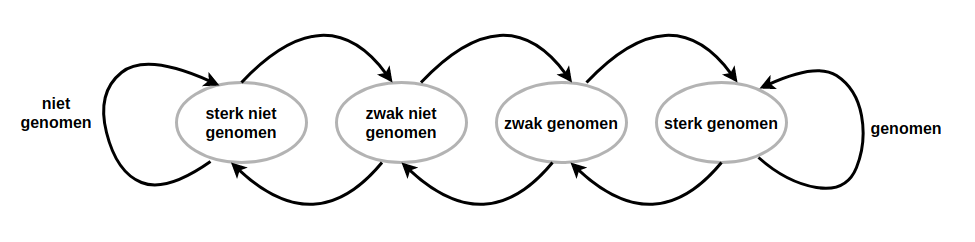
\includegraphics[width=1.0\linewidth]{img/predictor.png}
	\caption{2-bit teller}
	\label{fig:predictor}
\end{figure}

Een 2-bits verzadigde teller (ook bekend als een bimodale teller) is een status machine met vier staten: sterk niet genomen, zwak niet genomen, zwak genomen, sterk genomen. \parencite{Lee2017}
De 2-bits predictor (2BP, 2BC) heeft de volgende mogelijke waarden: 00, 01, 10, 11. Figuur \ref{fig:predictor} geeft een goed overzicht.

Het meest significante bit (eerste bit) van de predictor is de voorspelling zelf.
Dit wordt de voorspellingsbit genoemd.
De lagere bit (tweede bit) noemt de Hysteresis of Conviction bit.\\
Deze bit vertelt ons hoe zeker dat we zijn wat we moeten voorspellen.
Normaal gezien wordt de staat '00' behandeld als sterk niet genomen.
De eerste betekent niet genomen en we zijn redelijk overtuigd dat niet genomen het dominante gedrag is van deze branche.
De '01' staat is de zwak niet genomen staat. In deze staat zijn we niet zo zeker over het dominante gedrag.
Evenzo voor de genomen staat, hebben we de 'sterk genomen' en 'zwak genomen', respectievelijk '11' en '10'.



Wanneer een branch wordt onderzocht, wordt de bijhorende statusmachine bijgewerkt.
Branches die geëvalueerd worden als 'niet genomen' zullen de staat verlagen naar 'sterk niet genomen'.
In het geval dat de branch genomen wordt en de staat 'zwak genomen' is wordt de staat geüpdatet naar 'sterk genomen'.
Het voordeel van een 2-bit teller tegenover een één-bit teller is dat een branch twee keer moet afwijken als men de voorspelling wilt veranderen.

Een voorbeeld van een processor met een verzadigde teller is de eerste Intel Pentium.
\parencite{Fog2018}

Een tweevoudige branch predictor, ook wel 'correlation-based' predictor genoemd, gebruikt een tweedimensionale tabel.
Een tweedimensionale tabel met tellers wordt ook wel een Pattern History Tabel (PHT) genoemd.
Een rij in een Pattern History Table is bijvoorbeeld '1001'.
Een tweevoudige teller is niet verzadigd maar adaptief.
Als een conditionele statement drie keer uitgevoerd wordt, hangt de beslissing op de derde branche af van de vorige twee.

2-bits voorspellingsbufferschema's werken redelijk goed en zijn vrij eenvoudig te implementeren.
De MIPS R10000 processor uit 1996 heeft zo een schema en de nauwkeurigheid van de voorspellingen liggen rond de 90 procent.

Om deze reden is een tweevoudige adaptieve predictor beter dan een verzadigde teller.

Er zijn veel redenen waarom huidige branch predictors vrij accuraat zijn.
Een van die redenen is de distributie.
Individuele takken zijn vaak sterk bevooroordeeld ten opzichte van genomen of niet genomen.
Als de verdeling van de branches uniform zouden zijn (sterk niet genomen, zwak niet genomen, zwak genomen, sterk genomen) zou het veel moeilijker zijn om een goede branch predictor te maken.

Nog een reden is de afhankelijkheid tussen branches. In praktische programma's is er een sterke afhankelijkheid tussen verschillende branches. Dat wil zeggen dat de uitkomst van een branch de uitkomst van een andere branch beïnvloedt.

Branchevoorspelling is gebaseerd op de geschiedenis van
branches uitgevoerd tijdens de huidige uitvoering van
het programma.
De patrooninformatie over uitvoeringsgeschiedenis wordt tijdens het uitvoeren van een programma verzameld.
Daarom moet het programma niet vooraf gedraaid worden (ook gekend als pre-runs) 
\parencite{Yeh1991}.
Het tweevoudige adaptieve training schema heeft twee basis datastructuren: de Branch History Register (HR) en de Branch History Pattern table (HPT of PT), zoals beschreven in Lee en Smith \parencite{Lee1984}.

Met tweevoudige adaptieve training, in plaats van het bestuderen van de programma's zelf door het verzamelen van statistieken, wordt de uitvoeringsgeschiedenisinformatie verzameld door de geschiedenisregisters en de patroonbits in de PHT.

Nog een sub-unit is de 'Return Stack Buffer'. Deze buffer fungeert als een soort 'schaduw' stack.
Een schaduwstack is een mechanisme voor het beschermen van het opgeslagen retouradres van een procedure, zoals van een stackbuffer overflow.

Schaduwstacks kunnen worden geïmplementeerd door programma's met aangepaste prologen en epiloogpoorten opnieuw te compileren, door dynamische binaire herschrijftechnieken om hetzelfde effect te bereiken, of met hardware-ondersteuning \parencite{Sinnadurai2008}.

De return stack buffer slaat het retouradres voor 'CALL' instructies op, waardoor het doel van een RET-instructie beschikbaar wordt gesteld zonder dat de processor hoeft te vertrouwen op de BTB. Het is gedocumenteerd om 16 niveaus diep te zijn.
De grootte van de return stack buffer is meestal 4 - 16 ingangen.
De return stack buffer heeft 16 entries voor nabije terugkeeroperaties of 'near returns'.
De RSB is een LIFO-buffer met een vaste lengte
\parencite{Fog2018}
De return stack buffer wordt gereset bij een context switch.


\subsection{Branch Target Prediction}
Branch Prediction voorspelt of de branche al dan niet wordt genomen.
Branch Target Prediction voorspelt \emph{waar} de branche naar toe gaat.
Deze twee termen zijn onafhankelijk van elkaar.
Bijvoorbeeld een onvoorwaardelijke tak met een vast doel kan een oneindige lus, een 'goto' statement, een break of een niet-virtuele functieaanroep zijn.
Een onvoorwaardelijke branch met een variabel doel kan een return van een functie zijn, of een virtuele functie call, of een 'switch' statement.
Een conditionele branch met een vast doelwit kan een 'if' statement zijn, of de '\&\&' operator, of de '||' operator.

Een conditionele branch met een variabel doel kan een 'if' statement zijn.
Dit scenario is zeer uniek en heeft minder kans om te verschijnen onder normale omstandigheden.
Veel hangt af van de compiler of dit scenario opkomt.
De compiler kan één maken als een optimalisatie.
In dit geval is het een combinatie van de twee van de bovenstaande gevallen.
De beslissingen zijn tegengesteld, maar de predictors moeten dat niet zijn.

\subsection{Intel Branch Prediction Architectuur}
In Core 2 introduceerde Intel een structuur genaamd de Loop Stream Detector (LSD).
Loop Stream Detector is ontworpen om fetch en decode te vermijden voor lussen die kleiner zijn dan een bepaalde grootte.
De LSD bevindt zich in de BPU (Branch Prediction Unit) en het vertelt in feite aan de BPU om te stoppen met het voorspellen van branches.

Chips met een LSD maken het zelfs logisch om de lus niet uit te rollen (loop unrolling).
Loop unrolling is handig voor onderbrekingen veroorzaakt door afhankelijkheden (dependency stall) te vermijden.

Er zijn voornamelijk drie typen afhankelijkheden mogelijk in een processor. Dit zijn: structurele afhankelijkheid, beheersafhankelijkheid, gegevensafhankelijkheid \parencite{Hennessy2009}.

Een stall is een verloren cyclus in de pijplijn zonder nieuwe input.

Een structurele stall doet zich voor wanneer een deel van de capaciteit van de hardware nodig is door meerdere instructies tegelijkertijd.
De processor heeft dan conflicten met de hulpmiddelen in de pipeline.
Een goed voorbeeld is een enkele geheugeneenheid die zowel in de fetch toegankelijk is waar een instructie uit het geheugen wordt opgehaald, en de geheugenfase waarin gegevens worden geschreven en / of uit het geheugen worden gelezen \parencite{Hennessy2009}.
Dit kan opgelost worden door de caches te verdelen of een vertraging in de executie.




Het formaat is afhankelijk van het CPU-model.
Met Sandy Bridge was dit 28 micro-operaties. Het groeit tot 56 micro-operaties met Haswell en Broadwell. Het groeit weer met Skylake tot 64 micro-operaties. Dit is per thread.
Als Hyperthreading uit staat is er dubbel zoveel opslag.


Deze techniek spaart energie door de lus af te sluiten van de front end en verbetert prestaties door executie-eenheden vrij te maken.


Sinds Sandy Bridge is er een nieuwe cache: de gedecodeerde micro-operatie cache.
De cache slaat instructies op terwijl ze worden gedecodeerd.

Wanneer de fetch een nieuwe instructie neemt, controleert het eerst of het in de micro-operatie cache zit.
Als het in de cache zit zal het de rest van de pipeline overnemen en de branch predictor uitschakelen.
Een typische decoded micro-operatie cache kan 1,5K uops aan (1500 micro-operaties).
1.5K micro-ops is ongeveer zes kilobyte.

Kuops is een meting van het aantal operaties dat de processor kan opslaan, in plaats van het gebruik van de grootte in kilobytes.
Kilobytes kan wat misleidend zijn vanwege de verschillende instructies op elke cpu.

De cache zit in de L1 cache en is 'direct mapped'.
Directe mapping betekent dat elke geheugenlijn slechts in één cache-rij kan worden gebruikt.

De laatste bit van het geheugenadres bepaalt het cacheadres.
Dit is goedkoop om te implementeren, maar inefficiënt.
De cache is ook LRU (Least Recently Used).
Wanneer de cache vol is en meer ruimte vereist, zuivert het systeem het item met de laagste referentiefrequentie. \parencite{Lee2001}











\subsection{Timing aanval}
De Spectre aanval heeft veel variaties door het te combineren met andere technieken.
Met elke microcode patch zal een processor zich anders gaan gedragen en anders reageren tot een Spectre aanval.

\textbf{Evict+Time}

De Evict + Time-aanval werkt door het meten van de timing van bewerkingen die afhankelijk zijn van de
staat van de cache \parencite{Osvik2006}.
De bedoeling van Evict+Time is selectief de staat van de cache te manipuleren (bijvoorbeeld de data uit een volle cache set te verdrijven).
Een cache set kan bijvoorbeeld 4 cache lijnen bevatten.
Een cachelijn is in het algemeen gefixeerd in grootte, typisch 64 bytes.
Wanneer een cachelijn vanuit het geheugen naar de cache wordt gekopieerd, wordt er een cache-entry aangemaakt.

De Evict + Time aanval van Osvik et al. \parencite{Osvik2006} hebben de geheime sleutel met ongeveer 500.000
voorbeelden bij het aanvallen van OpenSSL op Athlon 64 kunnen terugkrijgen. Het verzamelen van de gegevens duurde ongeveer een halve minuut van continue metingen (\ref{fig:evicttime}).

Bernstein \parencite{Bernstein2005} beschrijft ook aanvallen op AES
die de variabiliteit in timing door cache-effecten kunnen exploiteren.
Zijn aanval kan gezien worden als een variant op de Evict+Time methode van Osvik et al.

Het grootste verschil is dat Bernstein \parencite{Bernstein2005} niet gebruik maakt van 
een expliciet model van de cache en actieve manipulatie. Bernstein gaat er van uit van het bestaan van
een aantal consistente, statistische timingspatronen als gevolg van verschillende effecten door geheugen access.
Het is simpeler maar heeft een paar nadelen.

Het heeft een referentiepunt nodig van encryptie onder een gekende sleutel in een identieke configuratie, en deze zijn vaak niet direct beschikbaar.
Zelfs wanneer de aanval van Bernstein \parencite{Bernstein2005} werkt, vereist dit
een veel groter aantal geanalyseerde coderingen.

Het lijkt onpraktisch op veel echte systemen vanwege te lage signaal-ruisverhouding.
Signaal-ruisverhouding betekent in het algemeen de verhouding van het signaalvermogen tot het ruisvermogen dat is opgenomen in een opname \parencite{Johnson2006}.

In het geval van deze code:
\begin{lstlisting}
if (condition == false)
read array1[Register1]
read [Register2]
\end{lstlisting}
Stel dat de branchpredictor denkt dat de conditie true is en dus verkeerd voorspeld.
Veronderstel dat de aanvaller een geheime waarde in Register1 wil weten.
De speculatieve executie zal array1[Register1] lezen, als het een cache hit is zal het lezen van Register2 snel van start gaan.


Als het lezen van array1[Register1] een cache miss is zal het lezen van het tweede register langer duren.
De timing van de aanval zal dus anders zijn.

\begin{figure}
	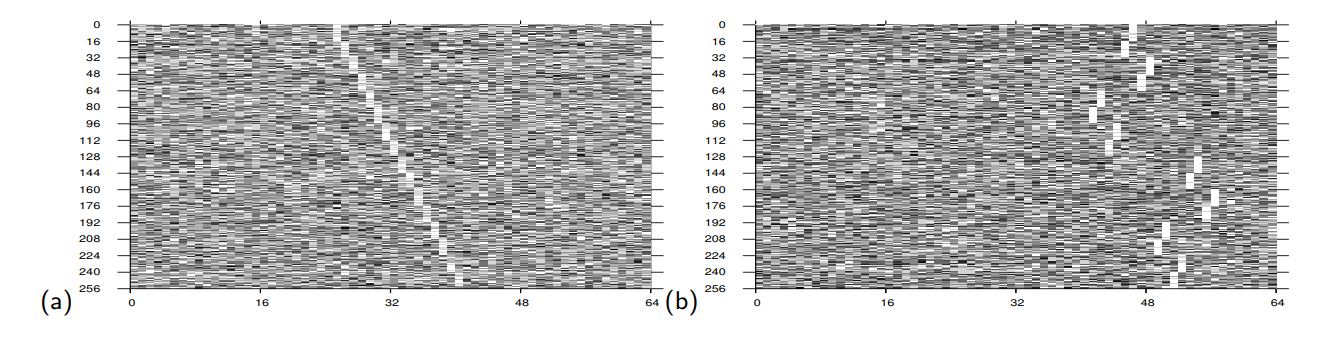
\includegraphics[width=1.0\linewidth]{img/evicttime.png}
	\caption{Evict+Time.}
	\label{fig:evicttime}
\end{figure}


\subsection{Branchscope}
Veiligheidsexperts hebben ontdekt dat Intel-chips kwetsbaar zijn voor een aanval die lijkt op Meltdown en Spectre.
In de nieuwe aanval past de aanvaller de PHT (Pattern History Table) aan.
De kwaadaardige code voert dan een branch uit die potentieel een verstoring kan veroorzaken in de PHT.
De aanvaller voert dan nog meer branches uit.

Als de aanvaller dan de storing in de PHT ziet kan hij/zij de branch aanpassen om de voorspelling te wijzigen.
Het directionele deel van de branch predictor (PHT) slaat een branch op (en de voorspelling dat genomen is).
De PHT is niet hetzelfde als de BTB.
De PHT is een ander onderdeel van de Branch Target Buffer (BTB).


De onderzoekers hebben alleen maar testen uitgevoerd op Intel-processors, en meer specifiek op Intel SGX (Software Guard Extensions).

Ze hebben AMD-chips niet getest, maar waarschijnlijk zullen ze er ook onder lijden.

Intel heeft gereageerd op de bevindingen en zelfs tezamen gewerkt met de onderzoekers.
Ze zeggen dat het onderzoek geloofwaardig is en dat de exploit vergelijkbaar is met eerder bekende side channel aanvallen.

Intel stelt ook vast dat bestaande softwarematige, risicobeperkende maatregelen, zoals side channel resistente cryptografie, ook effectief zijn tegen de methode in de paper.

\subsection{Branch Prediction}
Oude CPU's voeren één instructie uit per klokcyclus.
Instruction Level Parallelism (ILP) is een samenwerking van hardware en software om IPC te verbeteren. Hoe snel een programma presteert hangt af van beide: de CPU of de software zal de bottleneck zijn.
Voor betere snelheid werden 'pipelines' geïntroduceerd. Per klokcyclus werden meerdere delen van verschillende commando's uitgevoerd. 

De status wordt onthouden en overgedragen naar de volgende klokcyclus. Ondertussen kan er al een nieuwe pipeline gemaakt worden met nieuwe instructies. Deze verbetering in IPC (Instructies per klok) zorgt voor enkele problemen: een commando heeft het resultaat van een ander commando nodig maar is nog steeds in de pipeline, de programmalogica hangt af van een branch in de structuur. In het eerste geval kan de processor of eventueel software deze instructies 'out of order' uitvoeren zodat ze dichter bij elkaar liggen. In het tweede geval kan de CPU wachten op het resultaat maar dat kan honderden klokcyclussen duren. De predictor maakt een best mogelijke schatting van het resultaat en in het slechtste geval moet de voorspellende uitvoering  worden weggegooid.

Maar dit is typisch maar een verlies van een paar klokcyclussen.
Software kan ook IPC verbeteren: instructieplanning is een compiler optimalisatie om pipeline stall te vermijden.
Een pipeline stall is een vertraging in de pipeline om een probleem in de CPU architectuur op te lossen.
Dit gebeurt door de volgorde van instructies te herschikken.

Een simpele predictor voor speculatieve executie is de Branch Target Buffer (BTB). Het wordt gebruikt om vast te leggen of eerdere branches genomen werden of niet.
Het neemt de huidige PC (Program Counter) van de branch en gebruikt dat als een index in een tabel (de BTB) en van die tabel wordt de nieuwe PC voorspelt.
De Program Counter is een register in de CPU dat bijhoudt op welke instructie het momenteel is, het incrementeert telkens met de volgende instructie \parencite{Katzan1971}.

De nieuwe en de huidige PC worden mee in de pipeline genomen. Later in de pipeline hebben we de juiste PC en dan wordt de juiste PC met de voorspelde PC vergeleken. Als ze niet gelijk zijn is de voorspelling fout. De nieuwe PC wordt dan in de BTB tabel geschreven zodat de volgende confrontatie met de branch goed voorspeld wordt.
De BTB moet een volledig instructie-adres opslaan. Typisch is dat 64 bits of 8 bytes.

Speculatieve uitvoering verplicht de processor om gissingen te doen. Hoe beter het algoritme van de CPU, hoe meer prestaties. Een voorbeeld van branch prediction is een 'if statement' \parencite{Kocher2018}.
Er zijn schema's gebaseerd op de 'branch geschiedenis' om de beste voorspellingen te maken. Het voorspelde doelwit wordt opgeslagen in de branch target buffer.

Branch prediction wordt mogelijk gemaakt door een 'predictor', dat ingebakken zit in de processor.
Een moderne predictor gaat elke instructie speculatief uitvoeren, als het maar een branch instructie is.

De werking van speculatieve executie is een designkeuze van de fabrikant: een dure, performantie CPU kan agressievere speculatieve executie hebben dan een goedkopere uit dezelfde serie/architectuur.

De branch predictor leert van sprongen naar illegale
bestemmingen.
Hoewel een exception wordt gegooid in
het proces van de aanvaller, kan dit gemakkelijk worden gevangen (bijv.
met try ... catch)\parencite{Kocher2018}.



\section{Meltdown patch}
\subsection{Meltdown}
Meltdown omzeilt de door hardware afgedwongen isolatie van
beveiligingsdomeinen. Er is geen sprake van software-kwetsbaarheid
in Meltdown. Er is geen documentatie
of een dergelijke oplossing ontwikkeling van volledig
nieuwe hardware vereist, of kan worden opgelost met behulp van een microcode
update.

Omdat Meltdown misbruik maakt van out-of-order uitvoering, is het gemakkelijk opgelost
door out-of-order uitvoering volledig uit te schakelen. Maar, de prestatie-effecten
zouden groot zijn, omdat parallellisme van moderne CPU's
niet meer gebruikt kan worden. Dit is dus geen perfecte
oplossing.
Meltdown is een vorm van race-conditie tussen het
ophalen van een geheugenadres en de bijbehorende controle voor dit adres. De toestemming en de registerophaling serialiseren
kan Meltdown voorkomen,
aangezien het geheugenadres nooit wordt opgehaald als de permissiecontrole mislukt.




Dit brengt echter een aanzienlijke overhead met zich mee,
met elke fetch, omdat de fetch moet stoppen
totdat de machtigingscontrole is voltooid.
Een meer realistische oplossing zou zijn om een harde opsplitsing te introduceren
van gebruikersruimte en kernelruimte. Dit kan worden ingeschakeld door moderne kernels met een
bit in een CPU-register. Als de
bit is ingesteld, moet de kernelruimte zich in de eerste helft 
van de adresruimte bevinden, en de gebruikersruimte moet zich bevinden in 
de tweede helft van de adresruimte. Met deze splitsing, kan men onmiddellijk identificeren of een
fetch van de bestemming in strijd zou zijn met een permissie,
omdat het permissie-niveau rechtstreeks kan worden afgeleid van
het virtuele adres zonder verdere opzoekingen. Een dergelijke oplossing zou weinig impact hebben op performantie.

Verder is de achterwaartse compatibiliteit
verzekerd, omdat de kernel-bit niet standaard is ingesteld, en
de kernel stelt het alleen in als het de functie ondersteunt.
Merk op dat deze tegenmaatregelen alleen bij Meltdown voorkomen,
en niet bij de klasse van Spectre-aanvallen. 
Het is belangrijk om tegenmaatregelen in te zetten
tegen beide aanvallen.




\subsection{Statische analyse}
Statische code analyse wordt gebruikt om code sequenties te analyseren zonder het uit te voeren. Als de analyse code vindt met kwetsbare sequenties, zal het speculatieve executie uitschakelen tot alle code veilig uitgevoerd is.
Speculatieve executie wordt gestopt met een geheugenbarrière, ook bekend als een memory fence. Dit zijn extra instructies geschreven in machine code die de compiler dwingen om de instructies 'in order' te draaien.


\subsection{KPTI}
Hardware is alleen maar te patchen via softwarematige oplossingen totdat nieuwe hardware ontworpen kan worden.
De softwarematige oplossingen zijn in de vorm van microcode.
Microcode bepaalt de interne werking van een CPU.
De interne werking zit opgeslagen in een ROM (read-only memory).
Instructies worden als adressen aan deze ROM aangevoerd.
De ROM geeft controle signalen aan de andere componenten van de CPU, zoals de ALU (Rekenkundig-logische eenheid).

KPTI (ookwel PTI of KAISER genoemd) scheidt de kernelruimte van de gebruikersruimte af.
Deze wijziging was eerst bedoeld om side channel aanvallen te voorkomen, nu is het ook nuttig voor Meltdown.

De nieuwe releases van de Linux-kernel hebben volledige ondersteuning voor KPTI.
De patch zal ook oudere Linux-kernelversies ondersteunen. 
Natuurlijk hebben alle populaire besturingssystemen (Windows, Mac OS X, iOS, Android) dezelfde functies.

KPTI laat wel nog een aanvalsoppervlak achter, d.w.z. sommige geheugenlocaties kunnen nog steeds uitgelezen worden vanaf een gebruikersmodus. 
Deze geheugenlocaties bevatten geen belangrijke informatie zoals paswoorden, maar in het geval dat ze wijzen naar een ander adres via pointers, kunnen ze KPTI breken. 


Toch is KPTI momenteel de beste oplossing die beschikbaar is, en moet op alle systemen worden toegepast.
Zelfs met Meltdown kan KPTI kernelpointers
vermijden op geheugenlocaties
die in de gebruikersruimte in kaart zijn gebracht, en informatie zouden kunnen lekken. Dit zou 
trampolinelocaties vereisen voor elke kernel pointer.

Een trampolinefunctie springt in principe naar een instructie en laat die instructie meteen beslissen wat de volgende instructie is.
Een goed voorbeeld is een 'interrupt': de interrupt handler (een component van de CPU) weet niet echt hoe het met een evenement (bijvoorbeeld een toetsaanslag) moet omgaan, dus het laat de trampolinefunctie beslissen.


\section{Spectre patch}
\subsection{Retpoline}
Retpoline is een risicobeperkende maatregel voor Spectre variant 2 (CVE-2017-5715) gemaakt door Google.
Indirecte branches worden geconverteerd naar 'retpolines' in gevoelige code.
De spectre v2 aanval vergiftigt eerst de Branch Target Buffer (BTB) om daarna een adres te zoeken in gevoelige code.

Specifieker is retpoline gemaakt door Project Zero: een team van beveiligingsanalisten ingehuurd door Google gestart in 2014 \parencite{Evans2014}.
Retpoline is een manier om branch prediction teniet te doen.
Het is een nieuw concept om speculatieve executie uit te schakelen bij indirecte branches.
In praktijk wordt voor de x86 architectuur het geheugenadres in register 'r11' vervangen.


\begin{lstlisting}

jmp *%r11

call set_up_target;
capture_spec:         
pause;
jmp capture_spec;
set_up_target:
mov %r11, (%rsp);   
ret;    
\end{lstlisting}



\parencite{Turner2018}

Als de CPU nu code 'out of order' uitvoert zal het in een oneindige lus vastzitten. Het resultaat wordt niet teruggestuurd, dus het is niet zichtbaar door een aanvaller.
De lus wordt pas stopgezet als het echte resultaat teruggestuurd wordt.
Deze risicobeperkende maatregel is wel geen microcode patch. Software zal gehercompileerd moeten worden.

Retpoline is een soort ROP (Return Oriented Programming).\newline
Het idee van ROP  is om kwaadaardige code in de stack te injecteren door reeds bestaande codefragmenten te gebruiken.
Die fragmenten noemt de uitvinder van ROP (Hovav Shacham) gadgets. \parencite{Shacham2007}
ROP is een beveiligingsaanval maar in het geval van retpoline is het een beveiligingsverlichting (mitigation).
Een ROP instructie eindigt altijd met een return, vandaar de naam.


ROP is een extreme versie van 'stack smashing' of 'bufferoverloop'.
Bufferoverloop gebeurt wanneer er teveel functies aangeroepen worden, en er is niet genoeg ruimte meer in de stack. De stack heeft een hard limiet en op een gegeven moment kan er geen geheugen meer gealloceerd worden.
Stack bufferoverloop is gestopt door beveiligingen zoals NX (Never Execute) en Code Signing.
NX is een bit (no-execute bit) in gebieden van het geheugen en is geïmplementeerd in de Linux kernel sinds 2004.\parencite{KernelNewbies2004}
ROP kan deze systemen omzeilen.


De 'return' is een hardware instructie en vervangt traditionele 'jump' of 'call' instructie in systemen die gepatched zijn met 'retpoline'. Return instructies kunnen niet voorspeld worden door branch predictors dus een aanvaller kan geen geheugen uitlezen met een Spectre aanval.
Er zijn volledig afzonderlijke 'return buffers' dat de data opslaan. Als een aanvaller een voorspelling vergiftigd heeft wordt het omgezet in een return zonder voorspelling (en dus zonder prestatiewinst). Er zijn wel uitzonderingen met nieuwere Intel chips: in speciale situaties zal de branch target buffer nog steeds gebruikt worden.


Als een return van een geneste functie afkomstig is, kan de return buffer leeg gemaakt worden. De BTB zal dan toch gebruikt worden. Retpoline instructies kunnen dan een branch nemen dat gekozen is door een aanvaller. Intel zegt dat dit gebeurt op Broadwell of nieuwere processors en dat een microcode update dit probleem kan adresseren.
Omschakelen tussen virtuele machines kan ook voor problemen zorgen. De flags die Intel gebruikt voor Spectre (zoals IBPB, IBRS) moeten ingeschakeld zijn. De Linux kernel ondersteunt deze flags wel: bijvoorbeeld versie 4.16rc1.

\subsection{IBRS}


Indirect Branch Restricted Speculation (IBRS) verwijdert de cache tussen process modes en schakelt branch prediction uit voor 1 CPU kern (als de CPU hyperthreading heeft worden beide threads uitgeschakeld).

Dit gebeurt met een onderdeel van IBRS: Single Thread Indirect Branch Predictors (STIBP).
Als de processor IBRS niet ondersteund is moet software de \begin{verbatim}'IA32_SPEC_CTRL.IBRS'\end{verbatim}
bit instellen op 1.
Indirect Branch Prediction Barrier (IBPB) biedt een manier aan om de branch buffer opnieuw in te stellen en de status te verwijderen. AMD heeft ook microcode updates dat ongeveer hetzelfde werken als de 3 technieken van Intel.


Voor de nieuwste architectuur 'Zen' gebruikt AMD IPBP en STIBP. Voor oudere generaties zorgt de microcode voor IBRS en IBPB. De branch predictor van de nieuwe Ryzen, Threadripper en Epyc processors werkt anders en IBRS is daarom niet nodig. AMD zegt dat de nieuwe branch predictor niet op dezelfde manier kwetsbaar is. Oudere ontwerpen van BTB's (oudere AMD chips, Intel, ARM en Apple chips) gebruiken het volledig adres van de branch niet.
De BTB van Intel's Ivy Bridge en Haswell (en misschien zelfs Sandy Bridge) kunnen 4096 branches opslaan.\parencite{Godbolt2016}

Elke branch kan gemapt worden naar 4 mogelijke locaties in de BTB (4-voudig set associative).
In het geval van Haswell is het zelfs 5-voudig.
Het nadeel van deze techniek is dat een branch van één adres een branch van een ander adres kan beïnvloeden. Met een 4-voudige BTB kan 1 branch dus 4 locaties veranderen. In het geval van Spectre wordt de BTB vergiftigd door de aanvaller met foute adressen. Die adressen moeten niet volledig hetzelfde zijn, juist het gedeelte dat de BTB gebruikt. Wanneer de gebruiker dan een branch neemt zal het de uitkomst nemen dat is ingesteld door de aanvaller. AMD Zen chips kunnen alleen maar vergiftigd worden met een reëel, volledig adres.
De nieuwe micro-architectuur van Samsung, de Exynos M1, heeft ook een geavanceerdere branch predictor. Het gebruikt een 'perceptron' om de rate van branch hits te verbeteren.
Een perceptron is een 'algoritme voor gesuperviseerd leren van binaire classifiers (functies die kunnen bepalen of een invoer, weergegeven door een vector van getallen, behoort tot een bepaalde klasse of niet)'.\parencite{Freund1999}
Oftewel, het is een simpel neuraal netwerk. 
De Samsung Exynos M1 kan 2 branches per cyclus doen. Het concept van pipelining wordt dus in de predictor gebruikt.

Als de predictor tijdens een branch verkeerd gegokt heeft, moet de opgeslagen status opnieuw geladen worden en dat kan kostbare tijd innemen.
Branch prediction met perceptrons is niet nieuw: er zijn al veel studies rond gedaan en zelfs in oudere chips geïmplementeerd. Een van die chips is een AMD Trinity (A10-4600M) van 2012: de perceptron branch predictor werkte in parallel met de primaire branch predictor en had een aanvullende functie. 
Als de oude predictor en de nieuwe perceptron predictor over een branch van mening verschillen wordt het pad van de nieuwe predictor genomen.
Een conferentie uit 2001 demonstreerde dat een neurale predictor voorspellingsrates kan halen vergelijkbaar met conventionele, 2-niveau adaptieve predictors en dat neurale predictors verder onderzoek verdienen. \parencite{Steven2001}


De branch predictor van Zen gebruikt altijd het volledige adres van de branch.
Software moet wel herschreven worden om deze mechanismen te gebruiken.

\parencite{Intel2018}

\section{Geheugen Levels}
Processors gebruiken een hiërarchie van achtereenvolgend sneller wordende caches. Dit zijn de L1,L2,L3 caches.
Hoe lager het cacheniveau, hoe sneller de cache, maar hoe kleiner het is. Als een computer twee kernen heeft zal elke kern zijn eigen L1 en L2 cache hebben. Typisch is de L3 cache groot, maar die wordt gedeeld met alle kernen.

Een CPU bestaat uit registers, een Arithmetic Logic Unit (ALU) en een Control Unit. 
Met de localbus wordt een cache verbonden. De cache verstuurt data naar de register. 
De register stuurt data naar de ALU en die stuurt het resultaat naar de register, dan de cache, dan RAM. 
RAM verzendt het dan naar I/O apparaten of ander geheugen.

Voor de beste performantie zit de L1 cache in de kern zelf geëtst.
Ter vergelijking: L1, L2 en L3 hebben een vertraging van respectievelijk 3, 4, 21 en 87 klokcyclussen (AMD Bulldozer).

In systemen met meerderen kernen, aangezien er meer dan één L1/L2 cache is en elke cache een kopie van dezelfde gegevens kan bevatten, als deze in één kern wordt bijgewerkt moeten alle andere ook worden bijgewerkt.
Dit is waar het concept van 'valid bit' in beeld komt.
Tijdens het opstarten worden alle valid bits op 'invalid' gezet. De valid bit is na de markering gepositioneerd.
Als de markering hetzelfde is als het adres maar de valid bit is 0, wordt de ophaalactie als een 'cache miss' behandeld.

Een cache hit conditie is dus alleen voldaan als de markering gelijk is aan het geheugenbloknummer en de valid bit gelijk is aan 1. Door de initiële waarde van de valid bit op 0 te zetten kunnen er geen cache hits zijn voordat echte data opgehaald wordt.

Alle cacheniveaus van een moderne CPU zijn typisch n-way associatieve caches. Een associatieve cache met twee richtingen betekent dat elk hoofdgeheugenblok kan worden toegewezen aan een van twee cacheblokken. De L1 cache van de Piledriver architectuur is 2-way.\parencite{Hruska2017}
Hoe meer richtingen en hoe groter de cache, hoe hoger de hit-rate. L2 cache heeft daarom een hogere hit-rate dan L1.
Sommige processors hebben zelfs een L4 cache: bijvoorbeeld de Intel Core i7 4770R uit 2013 (128MB).

